\documentclass[conference]{IEEEtran}
\usepackage[T1]{fontenc}
\usepackage[utf8]{inputenc}
\usepackage[spanish,es-tabla]{babel}
\usepackage{graphicx,booktabs}
\title{Control colaborativo de precios e inventario con aprendizaje por refuerzo en Walmart M5}
\author{\IEEEauthorblockN{Leonardo Candio y Dimael Rivas}\IEEEauthorblockA{Universidad de Ingeniería y Tecnología\\ DS5345, Grupo 1}}
\begin{document}\maketitle
\begin{abstract}Estudiamos cómo coordinar precios y reposición cuando tres tiendas de California compiten por el mismo inventario regional. Sobre ventas y precios de Walmart M5 entrenamos Q-learning, Double DQN y PPO, y examinamos el efecto del diseño de la recompensa y de la experiencia sintética. En el último año, PPO superó el beneficio de la referencia inducida al 90 \% y redujo los quiebres en al menos 30 \% frente a ambas referencias en dos de tres semillas. Con cobertura al 95 \% ninguna política alcanzó el objetivo conjunto. La reposición inferida y la respuesta supuesta al precio condicionan la interpretación económica.\end{abstract}

\section*{I. Datos y proceso de decisión}
Usamos FOODS\_3\_090 en CA\_1, CA\_2 y CA\_3. Los tres CSV de M5 contienen ventas diarias, precios semanales y calendario [1]. Los días 1--1211 se usaron para entrenamiento, 1212--1576 para validación y 1577--1941 para el test de la campaña original. La revisión de la referencia histórica se hizo después de conocer ese último año.

El estado conjunto contiene el día, existencias locales y regionales, pedidos en tránsito e historial de ventas. Cada agente recibe una observación local, con calendario, precio base, stock regional, horizonte y pronóstico móvil de 28 días. Esta observación parcial limita la información para decidir. Cada tienda elige un multiplicador de precio entre 0,90 y 1,10 en pasos de 0,05 y una cobertura de 0, 3 o 7 días.

El pedido cubre la diferencia entre el objetivo y las existencias, sujeto a capacidad local. El centro distribuye hasta su inventario disponible en proporción a las solicitudes y resuelve los remanentes por tienda. Los despachos llegan al día siguiente. Las capacidades son 1050 unidades por tienda y 1768 regionales, con suministro diario máximo de 253.

\section*{II. Objetivo y agentes}
Con ventas históricas y, multiplicador m y elasticidad e, la demanda diaria simulada es el entero más próximo a y $\times$ m elevado a $-$e. Las ventas q están limitadas por las existencias disponibles. La recompensa regional suma, en las tres tiendas, precio $\times$ q menos 0,0128 por unidad almacenada al cierre y 1,28 por unidad perdida. Se reporta en unidades monetarias del simulador. M5 carece de costes de compra e inventarios diarios para este cálculo.

T0 reutiliza Q-learning de P1 con una tabla nueva por tienda y discretización de la observación. V0 aprende el valor de las acciones con Double DQN, replay y una red objetivo [2]. La red en línea elige la acción siguiente y la red objetivo la valora. P0 usa PPO con actores y críticos locales, clipping de 0,2 y GAE con parámetro 0,95 [3]. Los agentes cooperativos reciben el retorno regional. S0 aprende con la recompensa de su propia tienda.

\section*{III. Shaping potencial y Dyna}
Para cada tienda se calcula la cobertura como stock más tránsito, dividido por el pronóstico con mínimo uno y truncado a 14 días. El potencial $\Phi$ es el negativo de la suma de la varianza de cobertura dividida por 196 y el déficit medio de cobertura por debajo de tres días, dividido por tres. El potencial terminal vale cero.

Puesto que F = $\gamma$$\Phi$(s$'$) $-$ $\Phi$(s), sumar los términos descontados de F produce $-$$\Phi$(s$_0$) + $\gamma$$^{T}$$\Phi$(sT). En terminal, G$'$ = G $-$ $\Phi$(s$_0$). Para cualquier acción, Q* con shaping difiere de Q* base en la misma constante del estado inicial. El máximo conserva la misma acción [4]. En un ejemplo de dos pasos, servir supera a acaparar por 0,99 frente a 0,891. El bono ingenuo eleva acaparar a 1,881 e invierte el orden. PBRS conserva la preferencia por servir.

V1 incorpora PBRS, V2 incorpora Dyna y V3 combina ambos. N0 utiliza el bono ingenuo. Dyna aprende demanda a partir de observación, acción y tienda. Tras 256 transiciones reales, produce una transición sintética por paso elegible. El simulador calcula inventario y recompensa con sus ecuaciones contables.

\section*{IV. Comparación experimental}
Cada política se entrenó durante 300 episodios de 365 días con semillas 3, 4 y 5. Se congeló el checkpoint final. La incertidumbre entre semillas representa variación del aprendizaje sobre un mismo período comercial. Las bandas son desviaciones estándar muestrales. La evaluación económica excluye el shaping.

\begin{table}[!ht]\centering\footnotesize
\caption{Retorno medio y quiebres en el último año. H0 corresponde a la cobertura del 95 \%.}
\begin{tabular}{lrrrr}\toprule
Agente & Validación & Test & $\sigma$ test & Quiebres\\\midrule
H0 & 88 130 & 98 915 & --- & 1,26 \%\\
T0 & 85 477 & 98 649 & 635 & 2,21 \%\\
V0 & 84 938 & 97 144 & 1 496 & 4,77 \%\\
P0 & 86 092 & 96 590 & 536 & 1,33 \%\\
S0 & 71 698 & 74 439 & 42 056 & 10,06 \%\\
V1 & 83 149 & 96 796 & 4 584 & 4,63 \%\\
V2 & 76 522 & 90 553 & 11 668 & 8,80 \%\\
V3 & 81 906 & 94 290 & 2 288 & 5,12 \%\\
N0 & 84 218 & 97 658 & 3 366 & 3,89 \%\\
\bottomrule\end{tabular}
\end{table}
\begin{figure}[!ht]\centering
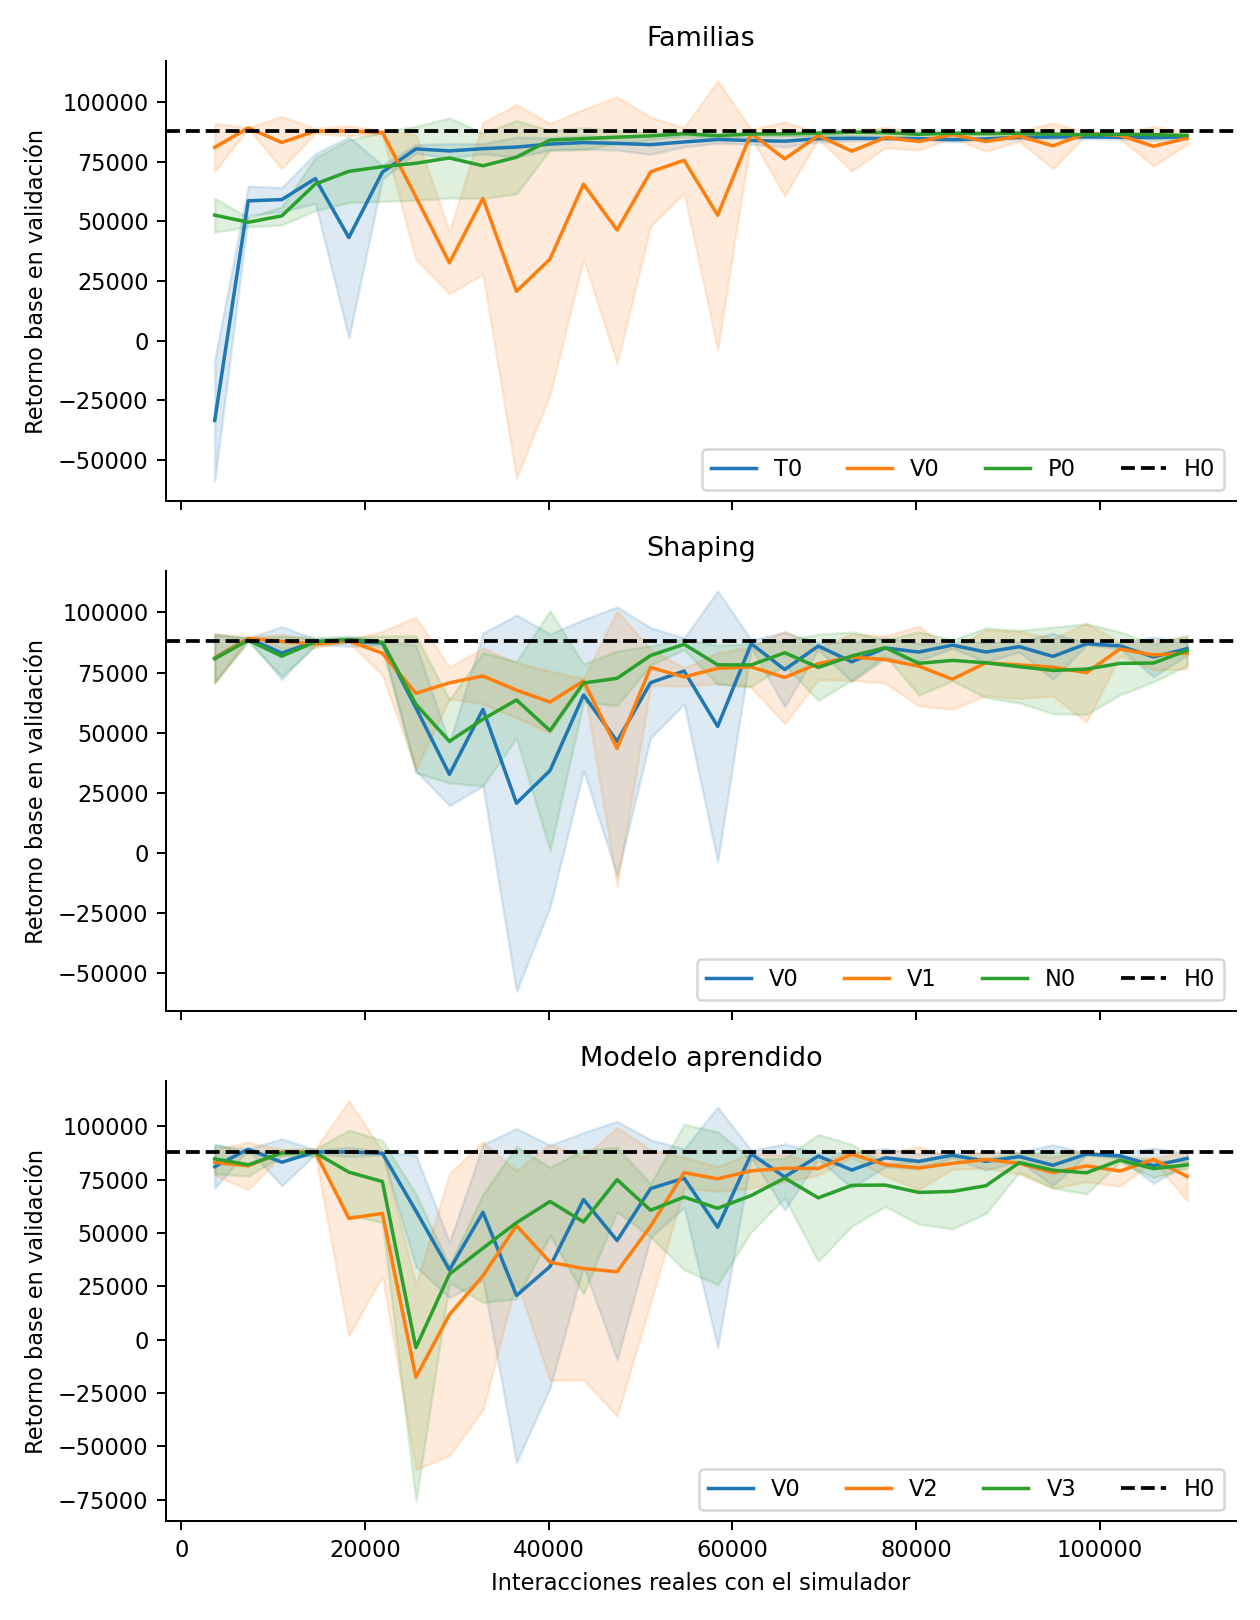
\includegraphics[width=\columnwidth,height=.36\textheight,keepaspectratio]{campana/validation_returns.png}
\caption{Retorno en validación según pasos reales. Cada panel compara una familia o una ablación con tres semillas.}
\end{figure}
\section*{Eficiencia muestral y estabilidad}
El umbral descriptivo es 72 143,5, el 80 \% del mayor retorno empírico de validación de la campaña. Se evalúa cada 3650 pasos. Las tres semillas de cada condición alcanzaron el umbral. La estabilidad se mide como dispersión entre episodios dentro de cada semilla y luego se promedia entre semillas.

\begin{table}[!ht]\centering\footnotesize
\caption{Mediana de pasos al umbral y desviación estándar de los últimos 30 episodios y 10 controles de validación.}
\begin{tabular}{lrrr}\toprule
Agente & Pasos & $\sigma$ entren. & $\sigma$ valid.\\\midrule
T0 & 14 600 & 19 077 & 573\\
V0 & 3 650 & 20 170 & 3 301\\
P0 & 18 250 & 20 366 & 794\\
S0 & 3 650 & 20 310 & 4 986\\
V1 & 3 650 & 20 018 & 5 560\\
V2 & 3 650 & 20 027 & 4 904\\
V3 & 3 650 & 20 564 & 7 600\\
N0 & 3 650 & 19 881 & 4 466\\
\bottomrule\end{tabular}
\end{table}
\begin{figure}[!ht]\centering
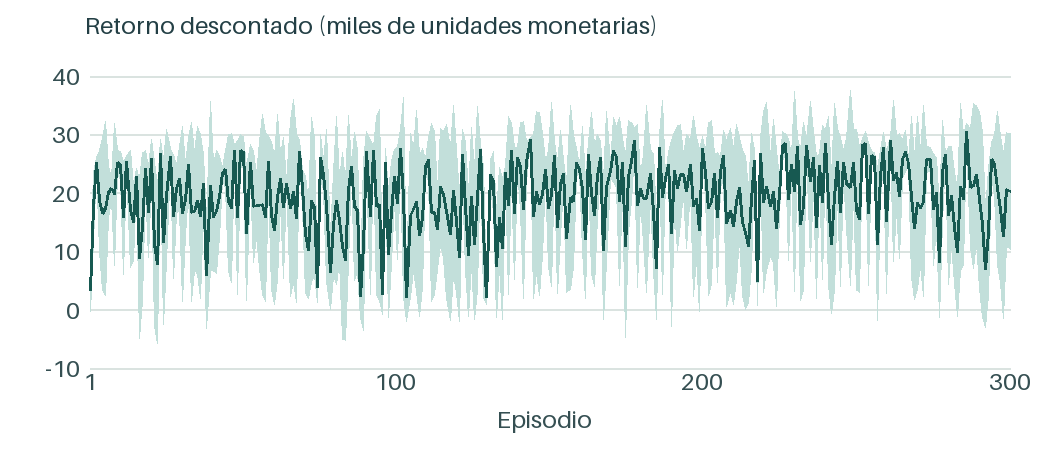
\includegraphics[width=\columnwidth,height=.36\textheight,keepaspectratio]{evidencia/g0_tabular.png}
\caption{Retorno descontado G$_0$ de Q-learning con $\gamma$ = 0,99, media $\pm$1$\sigma$. Se reprodujeron las tres semillas y coincidieron los 900 retornos episódicos sin descuento archivados.}
\end{figure}
\begin{figure}[!ht]\centering
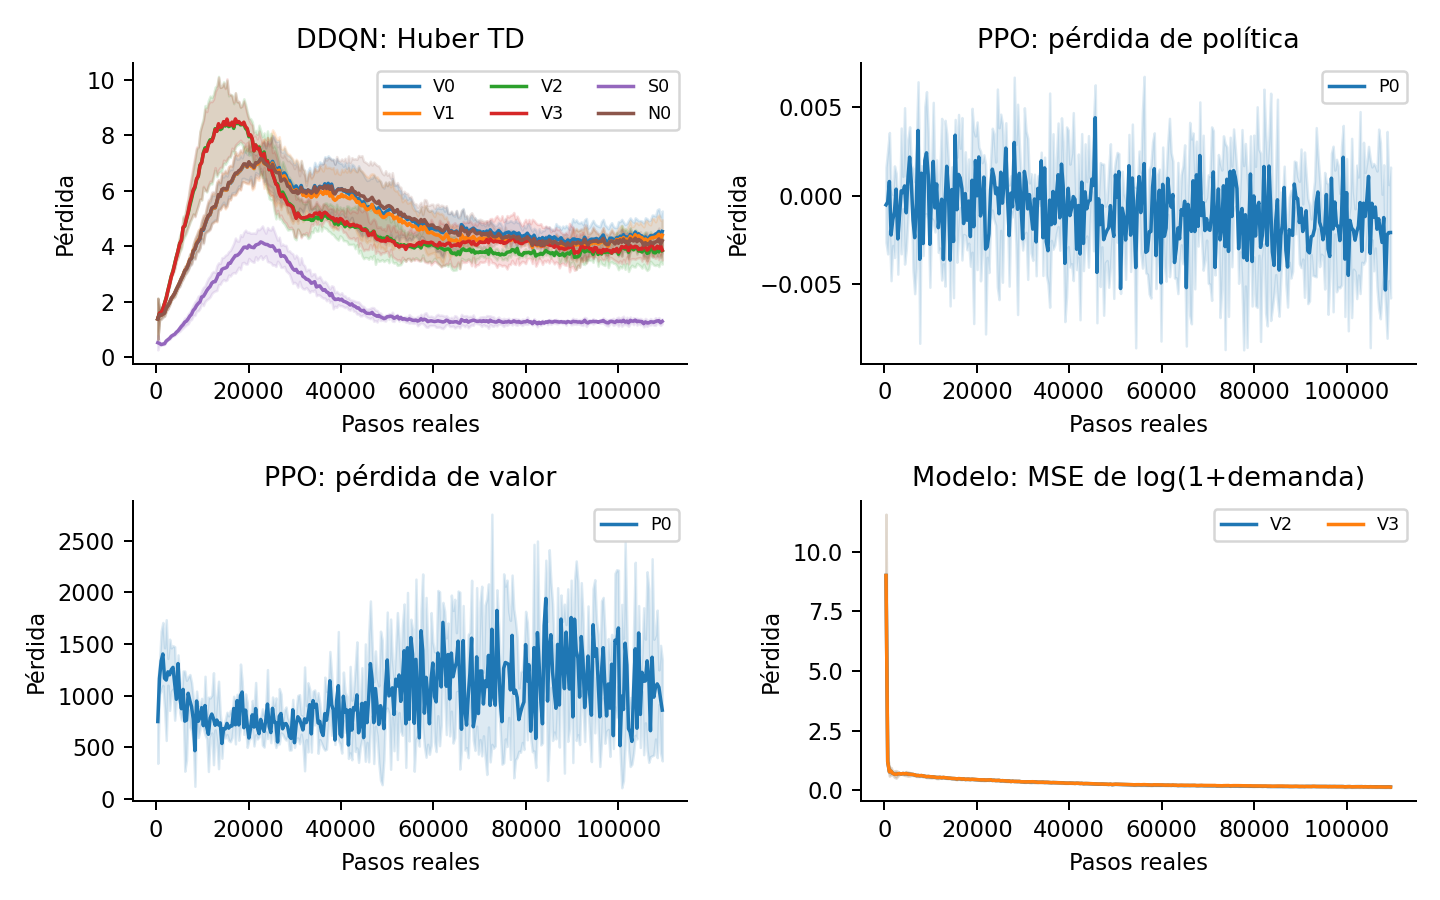
\includegraphics[width=\columnwidth,height=.36\textheight,keepaspectratio]{campana/losses_summary.png}
\caption{Pérdidas de entrenamiento por familia. Cada serie conserva su propia escala y tres semillas.}
\end{figure}
En los métodos profundos, los registros conservan el retorno acumulado sin descuento por episodio. La Fig. 4 muestra esa métrica. El G$_0$ descontado de estos métodos está disponible en test. La receta de reproducción registra ambos retornos en los entrenamientos futuros.

\section*{V. Referencia histórica inducida con M5}
Se fija el precio histórico y se elige por tienda la menor acción de reposición disponible que cubriría las ventas acumuladas de dos días en el porcentaje objetivo de ventanas de entrenamiento. Ese plazo comprende la decisión actual y el arribo del despacho. La cobertura deseada es un supuesto. La regla usa únicamente datos previos al período de evaluación.

\begin{table}[!ht]\centering\footnotesize
\caption{Efecto de la cobertura objetivo y comparación con PPO. Los objetivos se expresan en días para CA\_1, CA\_2 y CA\_3.}
\begin{tabular}{lrrrr}\toprule
Política & Objetivos & Ret. valid. & Ret. test & Quiebres$^{1}$\\\midrule
H0 90 \% & 7, 7, 3 & 54 777 & 83 354 & 11,88 \%\\
H0 95 \% & 7, 7, 7 & 88 130 & 98 915 & 1,26 \%\\
PPO & Aprendidos & 86 092 & 96 590 & 1,33 \%\\
\bottomrule\end{tabular}
\end{table}
$^{1}$ Tasa sobre días-tienda con demanda positiva en test. El retorno de PPO se promedia entre semillas. En CA\_3 el error absoluto medio de ventas en validación baja de 36,93 a 1,41 unidades diarias al pasar de tres a siete días de cobertura. Esto da respaldo empírico al escenario exigente, aunque las ventas observadas por sí solas admiten múltiples trayectorias de inventario.

\section*{Criterio conjunto por semilla}
Se requieren beneficio superior a H0 y reducción relativa de quiebres de al menos 30 \% frente a H0 y al egoísta S0 de la misma semilla. Para P0, elegida por retorno medio de validación, los resultados del escenario principal son los siguientes.

\begin{table}[!ht]\centering\footnotesize
\caption{PPO en test, frente a H0 al 90 \% y al control egoísta emparejado.}
\begin{tabular}{lrrrr}\toprule
Semilla & $\Delta$ retorno H0 & Red. H0 & Red. S0 & Cumple\\\midrule
3 & +13 195 & 87,61 \% & 94,42 \% & Sí\\
4 & +12 723 & 89,38 \% & 42,86 \% & Sí\\
5 & +13 792 & 89,38 \% & 20,00 \% & No\\
\bottomrule\end{tabular}
\end{table}
Al 90 \% cumplen 7 de 24 corridas de la matriz. Al 95 \% cumplen 0 de 24. El escenario del 95 \% reproduce la referencia original. Las dos coberturas formaron parte del reanálisis posterior de políticas congeladas. Este contraste utiliza un año de prueba ya examinado.

\section*{VI. Elasticidad, ablaciones y discusión}
Las políticas archivadas usaron e = 1,5 en las tres tiendas. Se estimó después, en entrenamiento, una regresión de Poisson por tienda con precio logarítmico, tendencia, estacionalidad, calendario y SNAP. Las elasticidades asociativas fueron 0,51, $-$1,73 y $-$1,49. Hubo entre 11 y 14 cambios de precio por tienda. La estimación común con tendencias por tienda pasó de $-$2,22 con 95 semanas a 2,20 con 173. La escasa variación de precio, los ceros y la disponibilidad desconocida limitan la identificación causal.

Al sustituir 1,5 por los tres coeficientes con sus signos observados en validación, T0 congelado de semilla 3 pasó de 86 419,91 a 83 022,89 de retorno y de 4,57 \% a 5,63 \% de quiebres. H0 conserva su trayectoria porque el multiplicador siempre es uno. Esta sensibilidad se ejecutó con la política tabular recuperada. Las cifras de PPO pertenecen al escenario original de elasticidad.

También se reentrenó Q-learning con los coeficientes asociativos de su propia tienda y las mismas tres semillas y 300 episodios. En el último año el retorno medio fue 103 248,36 y la tasa media de quiebres fue 2,28 \%. Este reanálisis conserva el período ya examinado. Las políticas egoístas calibradas son necesarias para medir la meta conjunta en ese entorno.

A igual número de interacciones reales, V1 obtuvo 348,7 unidades menos de retorno medio de test que V0, y V2 obtuvo 6591,5 menos. V3 recuperó 3737,4 frente a V2. Dyna redujo el MAE de demanda a 28,32 en V2 frente a 29,07 del pronóstico reciente, pero empeoró el RMSE. El menor error absoluto medio no aseguró mejor control. Una sola serie de producto y tres semillas limitan la generalización.

\begin{figure}[!ht]\centering
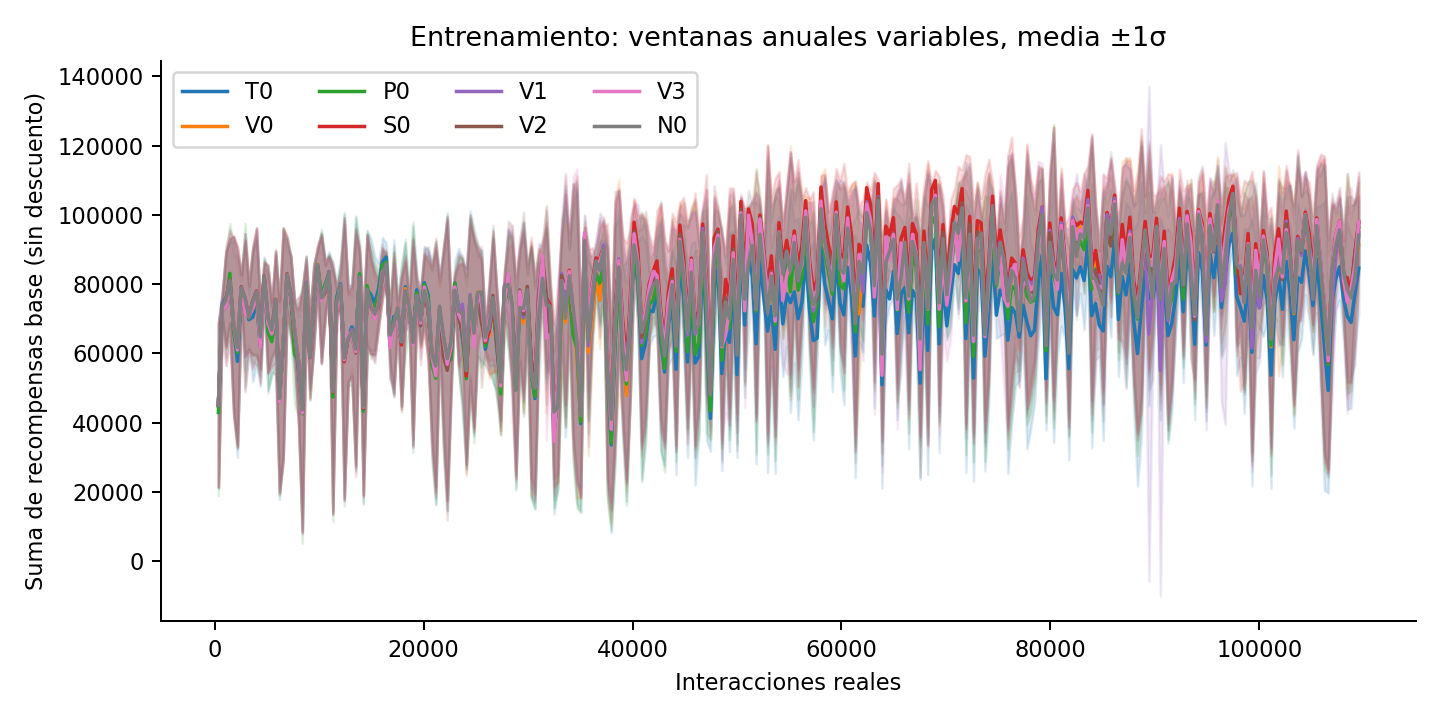
\includegraphics[width=\columnwidth,height=.36\textheight,keepaspectratio]{campana/training_returns.png}
\caption{Retorno episódico base sin descuento. Los episodios de entrenamiento abarcan ventanas distintas.}
\end{figure}
\section*{Referencias}
[1] University of Nicosia, M5 dataset, Zenodo, DOI 10.5281/zenodo.10203108. [2] H. van Hasselt et al., Deep Reinforcement Learning with Double Q-learning, AAAI, 2016. [3] J. Schulman et al., Proximal Policy Optimization Algorithms, 2017. [4] A. Ng et al., Policy Invariance Under Reward Transformations, ICML, 1999.

\end{document}